Nach erfolgreicher Einrichtung einer Cloud Node im IBM Spectrum Scale Cluster, kann diese nun mit unterschiedlichen Cloud Speichern verbunden werden.

Bei der Einrichtung wird davon ausgegangen, dass folgende Einstellungen vorgenommen wurden:
\begin{itemize}
	\item Name der NodeClass: \textbf{TCTNodeClass}
	\item Cloud Typ: \textbf{cleversafe-new}
	\item Cloud Bezeichnung: \textbf{mcstore}
	\item Name des Cloud-Dateisystems: \textbf{fs1}
\end{itemize}

Nach Hochfahren des Clusters kann mit \lstinline|mmhealth node show|, der Status der unterschiedlichen Dienste untersucht werden. Auf einer einzelnen Maschine kann es aber einige Minuten dauern, bis die Software vollständig hochgefahren ist.

Um den Zustand des Cloud Dienstes zu inspizieren, mit ihm zu arbeiten (Data Sharing / Cloud Tiering) oder ihn zu verändern wird das \lstinline|mmcloudgateway| Programm verwendet. Falls dieses nicht automatisch beim Systemstart initialisiert wird, kann es mithilfe von \lstinline|mmcloudgateway service start -N TCTNodeClass| manuell gestartet werden.

\begin{figure}[hbt]
	\centering
	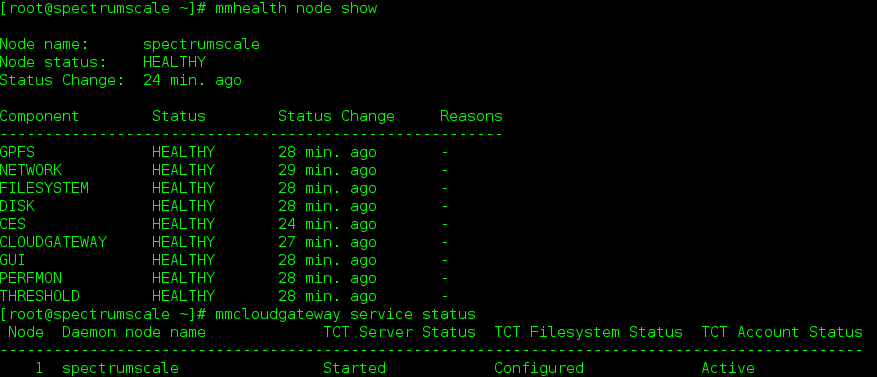
\includegraphics[scale=0.5]{images/scale-status}
	\caption{Beispielhafte Ausgabe von \lstinline|mmhealth| und \lstinline|mmcloudgateway| - mit konfiguriertem Cloudgateway}
	\label{fig:saclestatus}
\end{figure}


\textbf{Einrichtung des Cloud Data Sharing Accounts}\\
Als erstes muss die S3 Verbindung mit \ac{COS} hergestellt werden. Dafür sollte ein Verbindungstest der Account Daten im Vorhinein stattfinden, um spätere Probleme bei der Einrichtung zu verhindern.

Ein IBM Cloud Object Storage Account auf Softlayer kann unter dieser URL \url{https://www.ibm.com/cloud-computing/bluemix/cloud-object-storage} eingerichtet werden. 

Anschließend kann ein erster Bucket erstellt und Nutzername, Adresse des Endpunkts und Passwort von der Webseite ausgelesen werden. Hierbei gibt es Unterschiede bei der Befehlssyntax zwischen IBM Spectrum Scale und \ac{COS}. 
Der Nutzername wird bei S3 kompatiblen Schnittstellen normalerweise als \textit{AccessKeyId} und das Passwort als \textit{SecretAccessKey} bezeichnet. Bei IBM Spectrum Scale muss der \textit{SecretAccessKey} in eine Passwortdatei gespeichert und der \textit{AccessKeyId} als Nutzername (Username) übergeben werden.\\

\begin{lstlisting}[language=bash, caption=Vortest des Cloud Sharing Accounts]
mmcloudgateway account pre-test --cloud-type cleversafe-new --username "<username>" --pwd-file <path/file/your/secretAccessKey> --cloud-url <cos/endpoint>
\end{lstlisting}

Nach Ausführung obigen Befehls wird eine Testverbindung aufgebaut. Funktioniert dies fehlerfrei kann nun der Account eingerichtet werden. An dieser Stelle ist es extrem wichtig, dass die Option \lstinline|--enc-enable| auf \lstinline|FALSE| gesetzt wird. Ansonsten kann das beabsichtigte Cloud Data Sharing nicht umgesetzt werden, da beim Export eine Dateiverschlüsselung stattfindet. Diese macht das Lesen der Informationen von anderen Anwendungen (hier unsere Demoanwendung) unmöglich.

Die Befehlssyntax benötigt an dieser Stelle aber noch weitere Informationen, die für den Test nicht notwendig waren:\\

\begin{lstlisting}[language=bash, caption=Einrichtung des Cloud Sharing Accounts]
mmcloudgateway account create --cloud-nodeclass TCTNodeClass --cloud-name mcstore --cloud-type cleversafe-new --username "<username>" --pwd-file <path/file/your/secretAccessKey> --enable TRUE --cloud-url <cos/endpoint> --enc-enable FALSE
\end{lstlisting}

Nach erfolgreicher Ausführung des Befehls ist der Account fertig eingerichtet und man sollte die in \autoref{fig:saclestatus} gezeigte Ausgabe beim Überprüfen des Cloud Services sehen.

\textbf{Export von lokalen Dateien in die Cloud}\\
Um Informationen in den konfigurierten Cloud Account zu exportieren, muss zuerst in das ausgewählte Datei System für die Cloud Knoten gewechselt werden (hier: \lstinline|cd /gpfs/fs1|).

Mit dem bereits bekannten \lstinline|mmcloudgateway| Befehl können nun einzelne oder mehrere Dateien zwischen \ac{COS} und der lokalen Maschine kopiert werden.

Es besteht die Möglichkeit, Metadaten beim Data Sharing zu erhalten und alle exportierten Dateien in einem Manifest festzuhalten. Dieses hilft beim späteren Import, da eine Liste aller exportierten Dateien vorliegt. 

\begin{lstlisting}[language=bash, caption=Export von lokalen Dateien]
mmcloudgateway files export <path/to/file> --manifest-file manifest.txt --export-metadata
\end{lstlisting}

\begin{lstlisting}[language=bash, caption=Import von COS Dateien]
mmcloudgateway files import <fileKey> --import-metadata
\end{lstlisting}

Weitere Informationen hierzu befinden sich in \cite[S. 613]{scale.2017}.

\textbf{Erweiterung der IBM Spectrum Scale Funktionalität}\\
Da IBM Spectrum Scale keinerlei Kontrolle über die geteilten Daten hat, wird es auch nicht über mögliche neue Dateien informiert. Diese können also nativ nicht wieder importiert werden.

Um dies zu umgehen, gibt es zwei Möglichkeiten: Es kann ein kleiner Webserver auf einem IBM Spectrum Scale Knoten aufgesetzt werden, der von außen über Änderungen informiert wird und diese dann in das Manifest schreibt. Nachteil an dieser Lösung ist, dass zusätzliche Software für den Cluster entwicklet werden muss und diese auch immer nur auf einem Knoten läuft, was zu Leistungsengpässen führen kann.

Alternativ kann die Manifest Datei auch mit in den Cloudspeicher hochgeladen werden. Von hier kann eine Aktualisierung durch die Cloudanwendung (\autoref{sec:application}) geschehen, jedes Mal wenn neue Daten hinzugefügt werden. IBM Spectrum Scale kann nun immer als erstes die Manifest Datei wieder importieren und bekommt mit dieser dann Informationen über Dateiveränderungen.

Offensichtlich ist die zweite Lösung besser, da keine Veränderung am Cluster vorgenommen werden muss.